\section{Product perspective}
\label{sec:product_perspective}%

\subsection{Class Diagrams}
\label{subsec:class_diagrams}%
The diagram below represents and describes the classes involved in the system, their basic functionalities, attributes,
and the relationships between them.
From the diagram, it is easy to see how the tournament entity function as a bridge between different
components. More specifically, in our design we assigned to this entity the task to hold track 
of battles, leaderboard of the tournament itself and badge assignment.
All the other functionalities are esily understandable from within the diagram or 
will be later discussed. \newline
Here, we want to stress that, even though just an high level view of the system-to-be, some consideration of implementation can be done. 
More specifically, some design pattern can be taken into consideration:
\begin{itemize}
    \item Decorator Pattern: to implement the logic behind the scoring system. Educator's choice of different aspect to consider will be easily managable 
    \item Observer patter: to implement the structure behind the notification system.
    \item Factory pattern: for the creation of different Badges with different characteristics and requirements.
  \end{itemize}

\begin{figure}[H]
    \begin{center}
        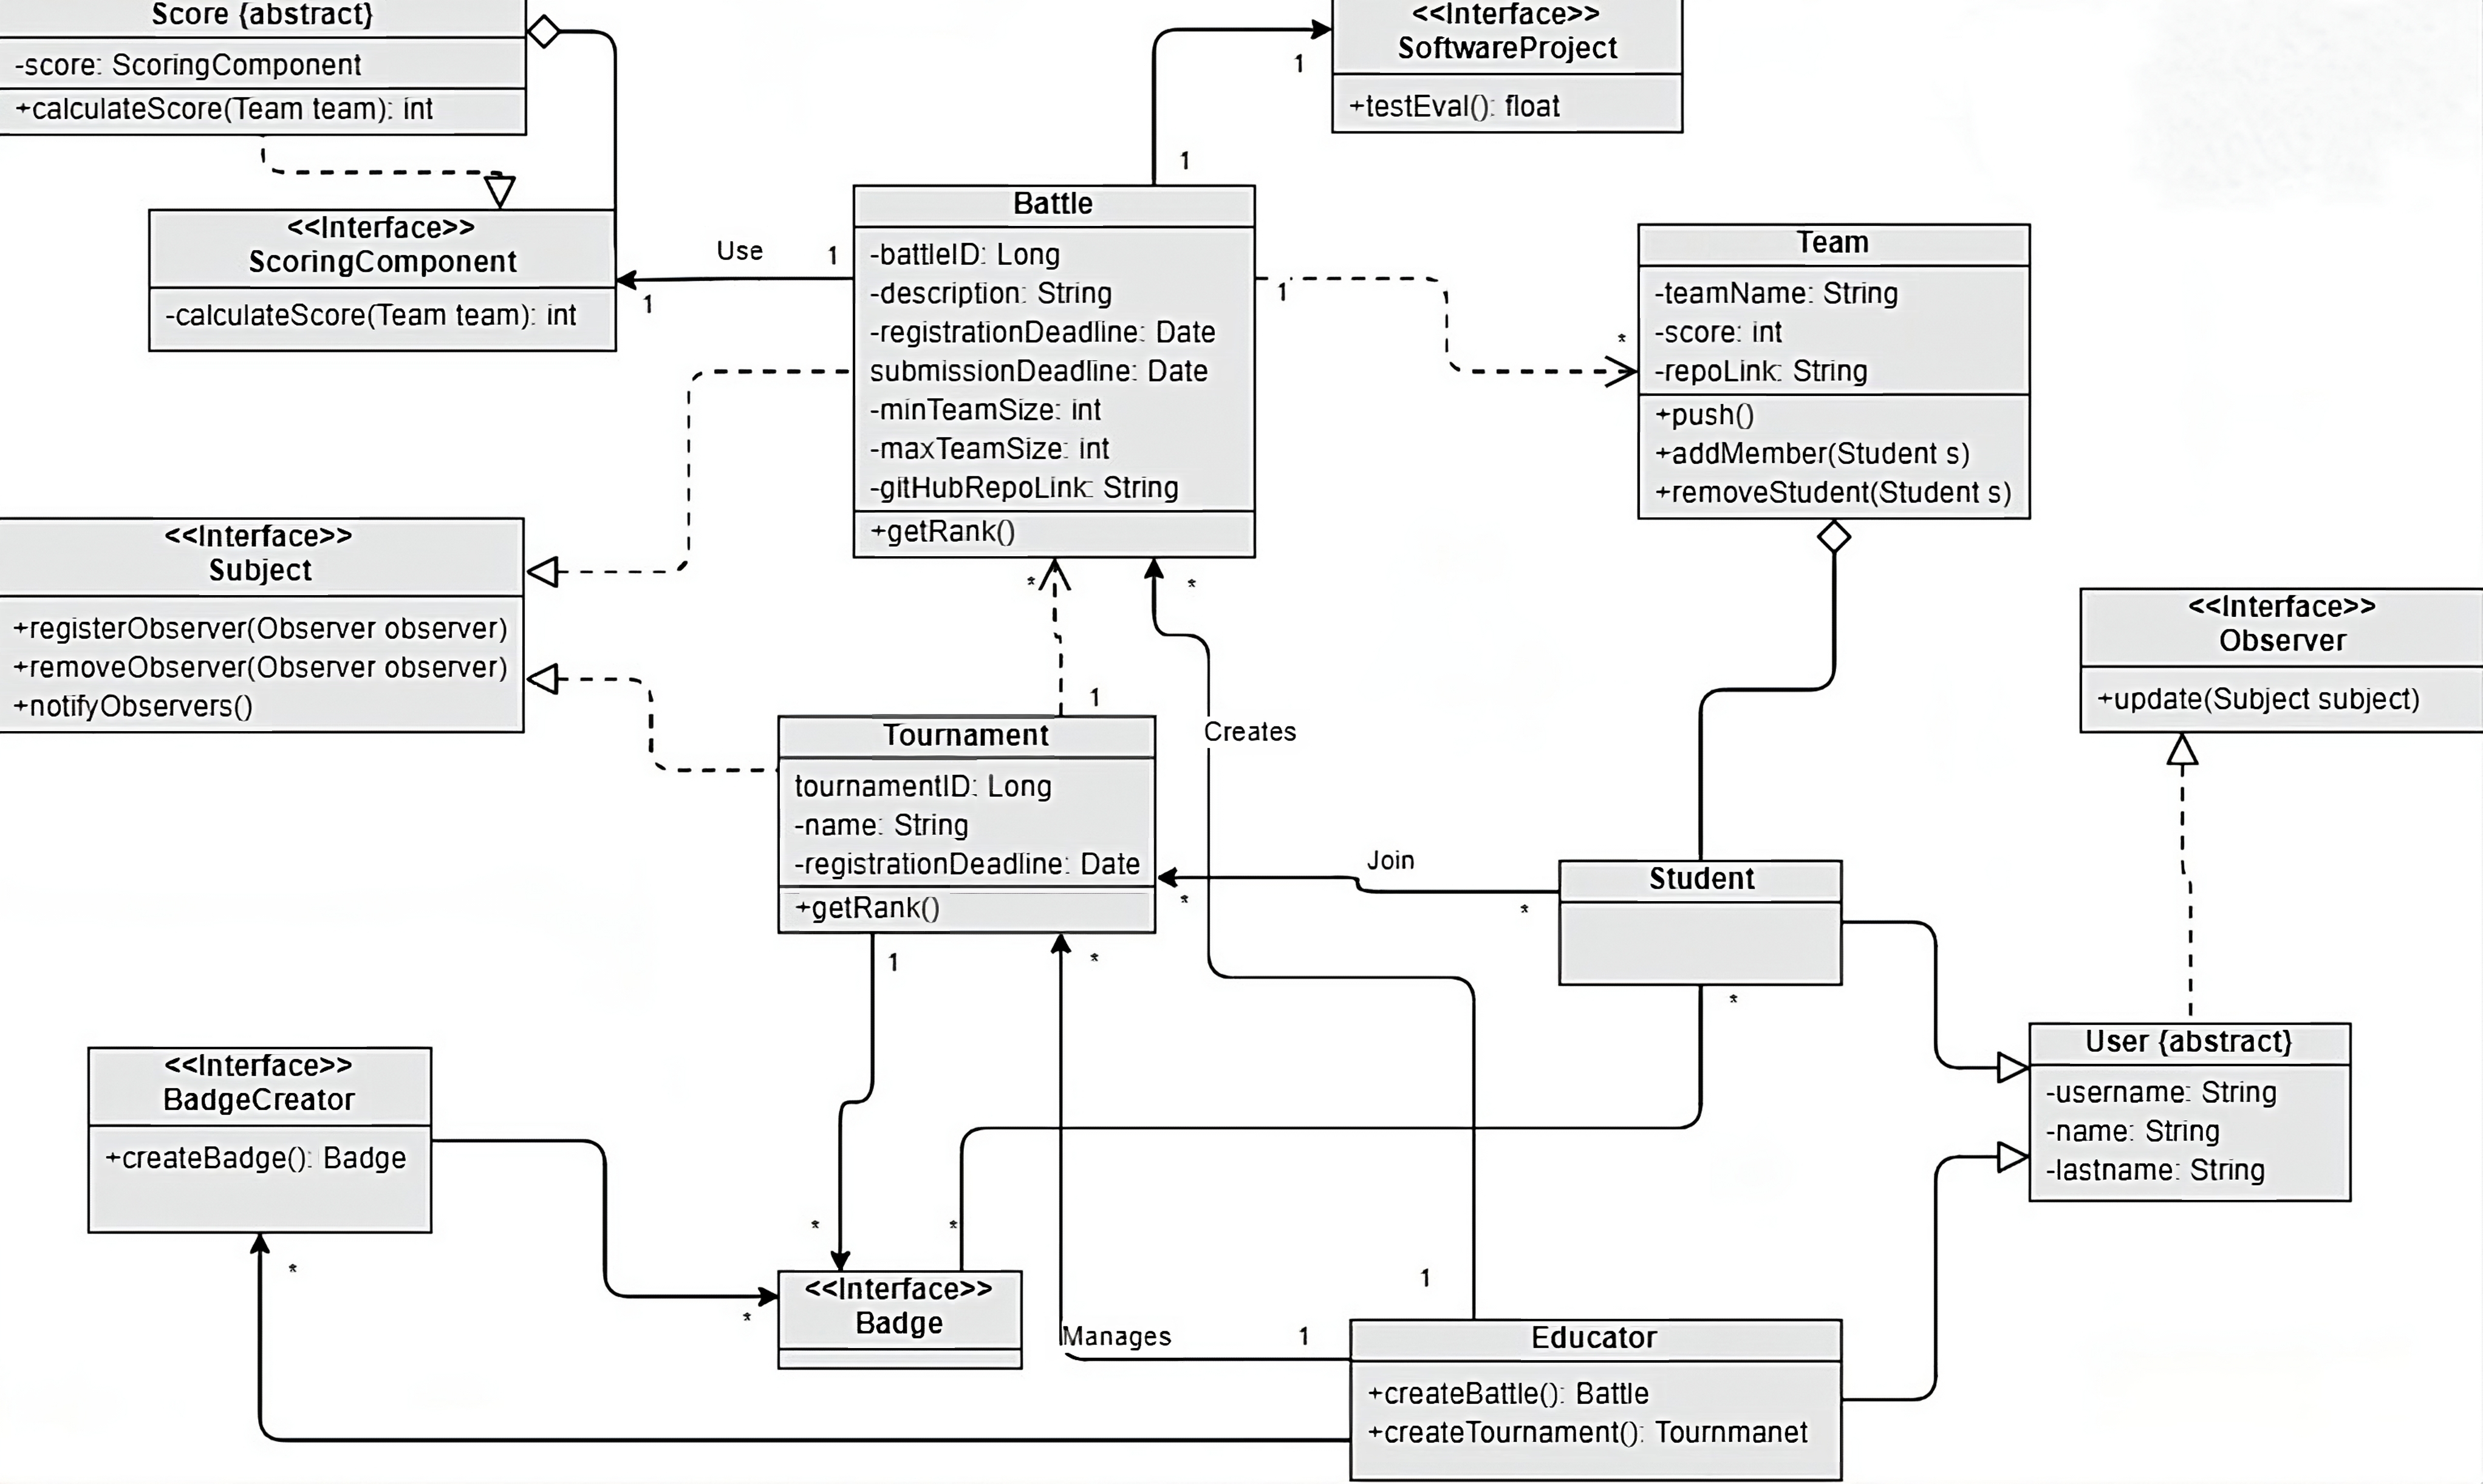
\includegraphics[width=0.9\linewidth]{Images/class-diagram.jpeg}
        \caption{A simplified Class Diagram}
        \label{fig:class_diagram}%
    \end{center}
\end{figure}

\subsection{State Diagrams}
\label{subsec:state_diagrams}%


\subsection{Scenarios}
\label{subsec:scenarios}%

\paragraph{Unregistered student creates an account.}
Gianmarco is a computer science student from Politecnico of Milan. After attending several courses about software engineering, 
he is looking for a way to practice his skills. Fortunately, one of his professor suggests him the CodeKataBattle CKB platform.
Gianmarco immediately proceeds to create an account. He navigates to the platform and goes to the "sign up" section. 
The system asks Gianmarco some personal information such as first and last name, an email linked 
to an institutional profile (for example name.surname@mail.polimi.it). He receives an e-mail with a 
6-digit code to be in inserted in the web page to confirm his e-mail address. In the meanwhile, the platform 
receives information about the status of Gianmarco from the university (whether he is a techer or a student). 
After accepting the terms \& conditions 
and submitting an username for his profile, the system creates his account, and Gianmarco can begin to use the platform.

\paragraph{Professor creates a tournament. }
Achille is a cyber security professor from university of Milan. He has an active profile on the CKB platform. 
During his last lesson, he annouced to his students that he will create monthly tournaments with weekly Battle for them to practise. 
He then proceeds to create the first tournament. He logs in the CKB platform from the "sign-in" page. 
Then, from the menu option in the home page, he selects "Create a new tournament". He is prompted with the page of the setup for the tournament itself. 
Achille enters a name for the tournament and the registration deadline. He then toggles the "advanced options" section. 
From here, he can decide wheter to include or not badges, and, in the first case, which badges are available in the tournament. 
Achille is prompted with a set of pre-existing badges (created from the platform or in previous tournaments). He can decide to 
create new badges in addition to the ones already present. When choosing to create a new badge, a pop-up window appears where he can select and combine 
variables and rules to obtain the new badge. Once he finishes setting up everything, he pushes the "Create tournament" button at the bottom of the page. 

\paragraph*{Professor closes a tournament.}
Logged into the CKB platform, Professor Lucia navigates to the "Tournaments" page. She locates the "Programming Prodigy Challenge" in the list and clicks
on it to access the tournament details. Satisfied with the students' participation and battle outcomes, she clicks the "Close Tournament" button.
A confirmation pop-up appears, and without hesitation, Professor Lucia confirms the action. The CKB platform processes the request, communicates 
the successful tournament closure, and computes the final ranking based on accumulated scores.
The platform promptly makes the final ranking available for participants. Professor Lucia, acknowledging the students' efforts, briefly reviews the rankings. 

\paragraph*{Professor creates a new CKB.}
Professor Roberto, logged into his CKB platform account, navigates to the tournament's details page named "Algorithmic Mastery Challenge." 
Excited to introduce a new coding challenge, he clicks on the "Create New Code Kata Battle" button. 
Professor Roberto is prompted to upload a code kata for the battle: he selects a well-prepared code kata that includes a comprehensive description and a software project with test cases and build automation scripts. 
He ensures that all necessary components are included before uploading.
Then he decides that groups should consist of a minimum of two students and a maximum of four students for this battle, so Professor Roberto sets these values accordingly in the "Group Size" field.
The educator proceeds to set a registration deadline and a final submission deadline, providing students with ample time to prepare and submit their solutions.
Curious about the advanced scoring options, Professor Roberto clicks on the "Additional Configurations for Scoring" button. 
The platform displays the scoring section, allowing him to set additional configurations if needed. 
Satisfied with the default scoring, he proceeds to click the "Create" button.

\paragraph*{Professor grants permissions to another professor to add CKB to a tournament.}
Professor Marta, logged into her CKB platform account, navigates to the details page of the tournament named "Coding Challenge Extravaganza," which she initiated. 
Realizing the workload involved in creating battles, she decides to grant permissions to another educator, Professor Elena.
She clicks on the "Add Administrator" button, prompting the CKB platform to request the email or username of the educator to whom she wants to grant permissions. 
Professor Marta confidently inputs Professor Elena's email.
Professor Elena receives a notification from the CKB platform, informing her that she has been granted permissions to add battles to the tournament named "Coding Challenge Extravaganza."
Now, Professor Elena, can access the tournament details page and contribute by creating new Code Kata Battles. 